
% Default to the notebook output style

    


% Inherit from the specified cell style.




    
\documentclass[11pt]{article}

    
    
    \usepackage[T1]{fontenc}
    % Nicer default font (+ math font) than Computer Modern for most use cases
    \usepackage{mathpazo}

    % Basic figure setup, for now with no caption control since it's done
    % automatically by Pandoc (which extracts ![](path) syntax from Markdown).
    \usepackage{graphicx}
    % We will generate all images so they have a width \maxwidth. This means
    % that they will get their normal width if they fit onto the page, but
    % are scaled down if they would overflow the margins.
    \makeatletter
    \def\maxwidth{\ifdim\Gin@nat@width>\linewidth\linewidth
    \else\Gin@nat@width\fi}
    \makeatother
    \let\Oldincludegraphics\includegraphics
    % Set max figure width to be 80% of text width, for now hardcoded.
    \renewcommand{\includegraphics}[1]{\Oldincludegraphics[width=.8\maxwidth]{#1}}
    % Ensure that by default, figures have no caption (until we provide a
    % proper Figure object with a Caption API and a way to capture that
    % in the conversion process - todo).
    \usepackage{caption}
    \DeclareCaptionLabelFormat{nolabel}{}
    \captionsetup{labelformat=nolabel}

    \usepackage{adjustbox} % Used to constrain images to a maximum size 
    \usepackage{xcolor} % Allow colors to be defined
    \usepackage{enumerate} % Needed for markdown enumerations to work
    \usepackage{geometry} % Used to adjust the document margins
    \usepackage{amsmath} % Equations
    \usepackage{amssymb} % Equations
    \usepackage{textcomp} % defines textquotesingle
    % Hack from http://tex.stackexchange.com/a/47451/13684:
    \AtBeginDocument{%
        \def\PYZsq{\textquotesingle}% Upright quotes in Pygmentized code
    }
    \usepackage{upquote} % Upright quotes for verbatim code
    \usepackage{eurosym} % defines \euro
    \usepackage[mathletters]{ucs} % Extended unicode (utf-8) support
    \usepackage[utf8x]{inputenc} % Allow utf-8 characters in the tex document
    \usepackage{fancyvrb} % verbatim replacement that allows latex
    \usepackage{grffile} % extends the file name processing of package graphics 
                         % to support a larger range 
    % The hyperref package gives us a pdf with properly built
    % internal navigation ('pdf bookmarks' for the table of contents,
    % internal cross-reference links, web links for URLs, etc.)
    \usepackage{hyperref}
    \usepackage{longtable} % longtable support required by pandoc >1.10
    \usepackage{booktabs}  % table support for pandoc > 1.12.2
    \usepackage[inline]{enumitem} % IRkernel/repr support (it uses the enumerate* environment)
    \usepackage[normalem]{ulem} % ulem is needed to support strikethroughs (\sout)
                                % normalem makes italics be italics, not underlines
    

    
    
    % Colors for the hyperref package
    \definecolor{urlcolor}{rgb}{0,.145,.698}
    \definecolor{linkcolor}{rgb}{.71,0.21,0.01}
    \definecolor{citecolor}{rgb}{.12,.54,.11}

    % ANSI colors
    \definecolor{ansi-black}{HTML}{3E424D}
    \definecolor{ansi-black-intense}{HTML}{282C36}
    \definecolor{ansi-red}{HTML}{E75C58}
    \definecolor{ansi-red-intense}{HTML}{B22B31}
    \definecolor{ansi-green}{HTML}{00A250}
    \definecolor{ansi-green-intense}{HTML}{007427}
    \definecolor{ansi-yellow}{HTML}{DDB62B}
    \definecolor{ansi-yellow-intense}{HTML}{B27D12}
    \definecolor{ansi-blue}{HTML}{208FFB}
    \definecolor{ansi-blue-intense}{HTML}{0065CA}
    \definecolor{ansi-magenta}{HTML}{D160C4}
    \definecolor{ansi-magenta-intense}{HTML}{A03196}
    \definecolor{ansi-cyan}{HTML}{60C6C8}
    \definecolor{ansi-cyan-intense}{HTML}{258F8F}
    \definecolor{ansi-white}{HTML}{C5C1B4}
    \definecolor{ansi-white-intense}{HTML}{A1A6B2}

    % commands and environments needed by pandoc snippets
    % extracted from the output of `pandoc -s`
    \providecommand{\tightlist}{%
      \setlength{\itemsep}{0pt}\setlength{\parskip}{0pt}}
    \DefineVerbatimEnvironment{Highlighting}{Verbatim}{commandchars=\\\{\}}
    % Add ',fontsize=\small' for more characters per line
    \newenvironment{Shaded}{}{}
    \newcommand{\KeywordTok}[1]{\textcolor[rgb]{0.00,0.44,0.13}{\textbf{{#1}}}}
    \newcommand{\DataTypeTok}[1]{\textcolor[rgb]{0.56,0.13,0.00}{{#1}}}
    \newcommand{\DecValTok}[1]{\textcolor[rgb]{0.25,0.63,0.44}{{#1}}}
    \newcommand{\BaseNTok}[1]{\textcolor[rgb]{0.25,0.63,0.44}{{#1}}}
    \newcommand{\FloatTok}[1]{\textcolor[rgb]{0.25,0.63,0.44}{{#1}}}
    \newcommand{\CharTok}[1]{\textcolor[rgb]{0.25,0.44,0.63}{{#1}}}
    \newcommand{\StringTok}[1]{\textcolor[rgb]{0.25,0.44,0.63}{{#1}}}
    \newcommand{\CommentTok}[1]{\textcolor[rgb]{0.38,0.63,0.69}{\textit{{#1}}}}
    \newcommand{\OtherTok}[1]{\textcolor[rgb]{0.00,0.44,0.13}{{#1}}}
    \newcommand{\AlertTok}[1]{\textcolor[rgb]{1.00,0.00,0.00}{\textbf{{#1}}}}
    \newcommand{\FunctionTok}[1]{\textcolor[rgb]{0.02,0.16,0.49}{{#1}}}
    \newcommand{\RegionMarkerTok}[1]{{#1}}
    \newcommand{\ErrorTok}[1]{\textcolor[rgb]{1.00,0.00,0.00}{\textbf{{#1}}}}
    \newcommand{\NormalTok}[1]{{#1}}
    
    % Additional commands for more recent versions of Pandoc
    \newcommand{\ConstantTok}[1]{\textcolor[rgb]{0.53,0.00,0.00}{{#1}}}
    \newcommand{\SpecialCharTok}[1]{\textcolor[rgb]{0.25,0.44,0.63}{{#1}}}
    \newcommand{\VerbatimStringTok}[1]{\textcolor[rgb]{0.25,0.44,0.63}{{#1}}}
    \newcommand{\SpecialStringTok}[1]{\textcolor[rgb]{0.73,0.40,0.53}{{#1}}}
    \newcommand{\ImportTok}[1]{{#1}}
    \newcommand{\DocumentationTok}[1]{\textcolor[rgb]{0.73,0.13,0.13}{\textit{{#1}}}}
    \newcommand{\AnnotationTok}[1]{\textcolor[rgb]{0.38,0.63,0.69}{\textbf{\textit{{#1}}}}}
    \newcommand{\CommentVarTok}[1]{\textcolor[rgb]{0.38,0.63,0.69}{\textbf{\textit{{#1}}}}}
    \newcommand{\VariableTok}[1]{\textcolor[rgb]{0.10,0.09,0.49}{{#1}}}
    \newcommand{\ControlFlowTok}[1]{\textcolor[rgb]{0.00,0.44,0.13}{\textbf{{#1}}}}
    \newcommand{\OperatorTok}[1]{\textcolor[rgb]{0.40,0.40,0.40}{{#1}}}
    \newcommand{\BuiltInTok}[1]{{#1}}
    \newcommand{\ExtensionTok}[1]{{#1}}
    \newcommand{\PreprocessorTok}[1]{\textcolor[rgb]{0.74,0.48,0.00}{{#1}}}
    \newcommand{\AttributeTok}[1]{\textcolor[rgb]{0.49,0.56,0.16}{{#1}}}
    \newcommand{\InformationTok}[1]{\textcolor[rgb]{0.38,0.63,0.69}{\textbf{\textit{{#1}}}}}
    \newcommand{\WarningTok}[1]{\textcolor[rgb]{0.38,0.63,0.69}{\textbf{\textit{{#1}}}}}
    
    
    % Define a nice break command that doesn't care if a line doesn't already
    % exist.
    \def\br{\hspace*{\fill} \\* }
    % Math Jax compatability definitions
    \def\gt{>}
    \def\lt{<}
    % Document parameters
    \title{Build a Stock Price Predictor}
    
    
    

    % Pygments definitions
    
\makeatletter
\def\PY@reset{\let\PY@it=\relax \let\PY@bf=\relax%
    \let\PY@ul=\relax \let\PY@tc=\relax%
    \let\PY@bc=\relax \let\PY@ff=\relax}
\def\PY@tok#1{\csname PY@tok@#1\endcsname}
\def\PY@toks#1+{\ifx\relax#1\empty\else%
    \PY@tok{#1}\expandafter\PY@toks\fi}
\def\PY@do#1{\PY@bc{\PY@tc{\PY@ul{%
    \PY@it{\PY@bf{\PY@ff{#1}}}}}}}
\def\PY#1#2{\PY@reset\PY@toks#1+\relax+\PY@do{#2}}

\expandafter\def\csname PY@tok@w\endcsname{\def\PY@tc##1{\textcolor[rgb]{0.73,0.73,0.73}{##1}}}
\expandafter\def\csname PY@tok@c\endcsname{\let\PY@it=\textit\def\PY@tc##1{\textcolor[rgb]{0.25,0.50,0.50}{##1}}}
\expandafter\def\csname PY@tok@cp\endcsname{\def\PY@tc##1{\textcolor[rgb]{0.74,0.48,0.00}{##1}}}
\expandafter\def\csname PY@tok@k\endcsname{\let\PY@bf=\textbf\def\PY@tc##1{\textcolor[rgb]{0.00,0.50,0.00}{##1}}}
\expandafter\def\csname PY@tok@kp\endcsname{\def\PY@tc##1{\textcolor[rgb]{0.00,0.50,0.00}{##1}}}
\expandafter\def\csname PY@tok@kt\endcsname{\def\PY@tc##1{\textcolor[rgb]{0.69,0.00,0.25}{##1}}}
\expandafter\def\csname PY@tok@o\endcsname{\def\PY@tc##1{\textcolor[rgb]{0.40,0.40,0.40}{##1}}}
\expandafter\def\csname PY@tok@ow\endcsname{\let\PY@bf=\textbf\def\PY@tc##1{\textcolor[rgb]{0.67,0.13,1.00}{##1}}}
\expandafter\def\csname PY@tok@nb\endcsname{\def\PY@tc##1{\textcolor[rgb]{0.00,0.50,0.00}{##1}}}
\expandafter\def\csname PY@tok@nf\endcsname{\def\PY@tc##1{\textcolor[rgb]{0.00,0.00,1.00}{##1}}}
\expandafter\def\csname PY@tok@nc\endcsname{\let\PY@bf=\textbf\def\PY@tc##1{\textcolor[rgb]{0.00,0.00,1.00}{##1}}}
\expandafter\def\csname PY@tok@nn\endcsname{\let\PY@bf=\textbf\def\PY@tc##1{\textcolor[rgb]{0.00,0.00,1.00}{##1}}}
\expandafter\def\csname PY@tok@ne\endcsname{\let\PY@bf=\textbf\def\PY@tc##1{\textcolor[rgb]{0.82,0.25,0.23}{##1}}}
\expandafter\def\csname PY@tok@nv\endcsname{\def\PY@tc##1{\textcolor[rgb]{0.10,0.09,0.49}{##1}}}
\expandafter\def\csname PY@tok@no\endcsname{\def\PY@tc##1{\textcolor[rgb]{0.53,0.00,0.00}{##1}}}
\expandafter\def\csname PY@tok@nl\endcsname{\def\PY@tc##1{\textcolor[rgb]{0.63,0.63,0.00}{##1}}}
\expandafter\def\csname PY@tok@ni\endcsname{\let\PY@bf=\textbf\def\PY@tc##1{\textcolor[rgb]{0.60,0.60,0.60}{##1}}}
\expandafter\def\csname PY@tok@na\endcsname{\def\PY@tc##1{\textcolor[rgb]{0.49,0.56,0.16}{##1}}}
\expandafter\def\csname PY@tok@nt\endcsname{\let\PY@bf=\textbf\def\PY@tc##1{\textcolor[rgb]{0.00,0.50,0.00}{##1}}}
\expandafter\def\csname PY@tok@nd\endcsname{\def\PY@tc##1{\textcolor[rgb]{0.67,0.13,1.00}{##1}}}
\expandafter\def\csname PY@tok@s\endcsname{\def\PY@tc##1{\textcolor[rgb]{0.73,0.13,0.13}{##1}}}
\expandafter\def\csname PY@tok@sd\endcsname{\let\PY@it=\textit\def\PY@tc##1{\textcolor[rgb]{0.73,0.13,0.13}{##1}}}
\expandafter\def\csname PY@tok@si\endcsname{\let\PY@bf=\textbf\def\PY@tc##1{\textcolor[rgb]{0.73,0.40,0.53}{##1}}}
\expandafter\def\csname PY@tok@se\endcsname{\let\PY@bf=\textbf\def\PY@tc##1{\textcolor[rgb]{0.73,0.40,0.13}{##1}}}
\expandafter\def\csname PY@tok@sr\endcsname{\def\PY@tc##1{\textcolor[rgb]{0.73,0.40,0.53}{##1}}}
\expandafter\def\csname PY@tok@ss\endcsname{\def\PY@tc##1{\textcolor[rgb]{0.10,0.09,0.49}{##1}}}
\expandafter\def\csname PY@tok@sx\endcsname{\def\PY@tc##1{\textcolor[rgb]{0.00,0.50,0.00}{##1}}}
\expandafter\def\csname PY@tok@m\endcsname{\def\PY@tc##1{\textcolor[rgb]{0.40,0.40,0.40}{##1}}}
\expandafter\def\csname PY@tok@gh\endcsname{\let\PY@bf=\textbf\def\PY@tc##1{\textcolor[rgb]{0.00,0.00,0.50}{##1}}}
\expandafter\def\csname PY@tok@gu\endcsname{\let\PY@bf=\textbf\def\PY@tc##1{\textcolor[rgb]{0.50,0.00,0.50}{##1}}}
\expandafter\def\csname PY@tok@gd\endcsname{\def\PY@tc##1{\textcolor[rgb]{0.63,0.00,0.00}{##1}}}
\expandafter\def\csname PY@tok@gi\endcsname{\def\PY@tc##1{\textcolor[rgb]{0.00,0.63,0.00}{##1}}}
\expandafter\def\csname PY@tok@gr\endcsname{\def\PY@tc##1{\textcolor[rgb]{1.00,0.00,0.00}{##1}}}
\expandafter\def\csname PY@tok@ge\endcsname{\let\PY@it=\textit}
\expandafter\def\csname PY@tok@gs\endcsname{\let\PY@bf=\textbf}
\expandafter\def\csname PY@tok@gp\endcsname{\let\PY@bf=\textbf\def\PY@tc##1{\textcolor[rgb]{0.00,0.00,0.50}{##1}}}
\expandafter\def\csname PY@tok@go\endcsname{\def\PY@tc##1{\textcolor[rgb]{0.53,0.53,0.53}{##1}}}
\expandafter\def\csname PY@tok@gt\endcsname{\def\PY@tc##1{\textcolor[rgb]{0.00,0.27,0.87}{##1}}}
\expandafter\def\csname PY@tok@err\endcsname{\def\PY@bc##1{\setlength{\fboxsep}{0pt}\fcolorbox[rgb]{1.00,0.00,0.00}{1,1,1}{\strut ##1}}}
\expandafter\def\csname PY@tok@kc\endcsname{\let\PY@bf=\textbf\def\PY@tc##1{\textcolor[rgb]{0.00,0.50,0.00}{##1}}}
\expandafter\def\csname PY@tok@kd\endcsname{\let\PY@bf=\textbf\def\PY@tc##1{\textcolor[rgb]{0.00,0.50,0.00}{##1}}}
\expandafter\def\csname PY@tok@kn\endcsname{\let\PY@bf=\textbf\def\PY@tc##1{\textcolor[rgb]{0.00,0.50,0.00}{##1}}}
\expandafter\def\csname PY@tok@kr\endcsname{\let\PY@bf=\textbf\def\PY@tc##1{\textcolor[rgb]{0.00,0.50,0.00}{##1}}}
\expandafter\def\csname PY@tok@bp\endcsname{\def\PY@tc##1{\textcolor[rgb]{0.00,0.50,0.00}{##1}}}
\expandafter\def\csname PY@tok@fm\endcsname{\def\PY@tc##1{\textcolor[rgb]{0.00,0.00,1.00}{##1}}}
\expandafter\def\csname PY@tok@vc\endcsname{\def\PY@tc##1{\textcolor[rgb]{0.10,0.09,0.49}{##1}}}
\expandafter\def\csname PY@tok@vg\endcsname{\def\PY@tc##1{\textcolor[rgb]{0.10,0.09,0.49}{##1}}}
\expandafter\def\csname PY@tok@vi\endcsname{\def\PY@tc##1{\textcolor[rgb]{0.10,0.09,0.49}{##1}}}
\expandafter\def\csname PY@tok@vm\endcsname{\def\PY@tc##1{\textcolor[rgb]{0.10,0.09,0.49}{##1}}}
\expandafter\def\csname PY@tok@sa\endcsname{\def\PY@tc##1{\textcolor[rgb]{0.73,0.13,0.13}{##1}}}
\expandafter\def\csname PY@tok@sb\endcsname{\def\PY@tc##1{\textcolor[rgb]{0.73,0.13,0.13}{##1}}}
\expandafter\def\csname PY@tok@sc\endcsname{\def\PY@tc##1{\textcolor[rgb]{0.73,0.13,0.13}{##1}}}
\expandafter\def\csname PY@tok@dl\endcsname{\def\PY@tc##1{\textcolor[rgb]{0.73,0.13,0.13}{##1}}}
\expandafter\def\csname PY@tok@s2\endcsname{\def\PY@tc##1{\textcolor[rgb]{0.73,0.13,0.13}{##1}}}
\expandafter\def\csname PY@tok@sh\endcsname{\def\PY@tc##1{\textcolor[rgb]{0.73,0.13,0.13}{##1}}}
\expandafter\def\csname PY@tok@s1\endcsname{\def\PY@tc##1{\textcolor[rgb]{0.73,0.13,0.13}{##1}}}
\expandafter\def\csname PY@tok@mb\endcsname{\def\PY@tc##1{\textcolor[rgb]{0.40,0.40,0.40}{##1}}}
\expandafter\def\csname PY@tok@mf\endcsname{\def\PY@tc##1{\textcolor[rgb]{0.40,0.40,0.40}{##1}}}
\expandafter\def\csname PY@tok@mh\endcsname{\def\PY@tc##1{\textcolor[rgb]{0.40,0.40,0.40}{##1}}}
\expandafter\def\csname PY@tok@mi\endcsname{\def\PY@tc##1{\textcolor[rgb]{0.40,0.40,0.40}{##1}}}
\expandafter\def\csname PY@tok@il\endcsname{\def\PY@tc##1{\textcolor[rgb]{0.40,0.40,0.40}{##1}}}
\expandafter\def\csname PY@tok@mo\endcsname{\def\PY@tc##1{\textcolor[rgb]{0.40,0.40,0.40}{##1}}}
\expandafter\def\csname PY@tok@ch\endcsname{\let\PY@it=\textit\def\PY@tc##1{\textcolor[rgb]{0.25,0.50,0.50}{##1}}}
\expandafter\def\csname PY@tok@cm\endcsname{\let\PY@it=\textit\def\PY@tc##1{\textcolor[rgb]{0.25,0.50,0.50}{##1}}}
\expandafter\def\csname PY@tok@cpf\endcsname{\let\PY@it=\textit\def\PY@tc##1{\textcolor[rgb]{0.25,0.50,0.50}{##1}}}
\expandafter\def\csname PY@tok@c1\endcsname{\let\PY@it=\textit\def\PY@tc##1{\textcolor[rgb]{0.25,0.50,0.50}{##1}}}
\expandafter\def\csname PY@tok@cs\endcsname{\let\PY@it=\textit\def\PY@tc##1{\textcolor[rgb]{0.25,0.50,0.50}{##1}}}

\def\PYZbs{\char`\\}
\def\PYZus{\char`\_}
\def\PYZob{\char`\{}
\def\PYZcb{\char`\}}
\def\PYZca{\char`\^}
\def\PYZam{\char`\&}
\def\PYZlt{\char`\<}
\def\PYZgt{\char`\>}
\def\PYZsh{\char`\#}
\def\PYZpc{\char`\%}
\def\PYZdl{\char`\$}
\def\PYZhy{\char`\-}
\def\PYZsq{\char`\'}
\def\PYZdq{\char`\"}
\def\PYZti{\char`\~}
% for compatibility with earlier versions
\def\PYZat{@}
\def\PYZlb{[}
\def\PYZrb{]}
\makeatother


    % Exact colors from NB
    \definecolor{incolor}{rgb}{0.0, 0.0, 0.5}
    \definecolor{outcolor}{rgb}{0.545, 0.0, 0.0}



    
    % Prevent overflowing lines due to hard-to-break entities
    \sloppy 
    % Setup hyperref package
    \hypersetup{
      breaklinks=true,  % so long urls are correctly broken across lines
      colorlinks=true,
      urlcolor=urlcolor,
      linkcolor=linkcolor,
      citecolor=citecolor,
      }
    % Slightly bigger margins than the latex defaults
    
    \geometry{verbose,tmargin=1in,bmargin=1in,lmargin=1in,rmargin=1in}
    
    

    \begin{document}
    
    
    \maketitle
    
    

    
    \section{Capstone Proposal}\label{capstone-proposal}

\begin{verbatim}
Dang Le Dang Khoa
April 17th, 2018
\end{verbatim}

\section{Domain Background}\label{domain-background}

\begin{itemize}
\item
  Investment firms, hedge funds, and even individuals have been using
  financial models to better understand market behavior and make
  profitable investments and trades. A wealth of information is
  available in the form of historical stock prices and company
  performance data, suitable for machine learning algorithms to process.
\item
  For this project, the task is to build a stock price predictor that
  takes daily trading data over a certain date range as input, and
  outputs projected estimates for given query dates. Note that the
  inputs will contain multiple metrics, such as opening price (Open),
  highest price the stock traded at (High), how many stocks were traded
  (Volume) and closing price adjusted for stock splits and dividends
  (Adjusted Close); the system only needs to predict the Adjusted Close
  price.
\end{itemize}

\section{Problem Statement}\label{problem-statement}

\begin{itemize}
\tightlist
\item
  Predict(forecast) the Adjusted Close day by day
\item
  Suggest 2 different approaches:

  \begin{itemize}
  \tightlist
  \item
    Traditional supervised machine learning methods(Regressions)
  \item
    A specific machine learning method for time series forecasting(ARIMA
    model)
  \end{itemize}
\item
  Challenges of Time series data:

  \begin{itemize}
  \tightlist
  \item
    Contains a lot of noises
  \item
    Is different from tabular data that each data point related to each
    other
  \item
    Contains time-dependent structures:

    \begin{itemize}
    \tightlist
    \item
      Level: the average value in the series
    \item
      Trend: global increasing or decreasing
    \item
      Seasonalities: repeating pattern of the series
    \end{itemize}
  \end{itemize}
\end{itemize}

\section{Datasets and Inputs}\label{datasets-and-inputs}

\begin{itemize}
\tightlist
\item
  Dataset downloaded from: \url{http://finance.yahoo.com}
\item
  Example: GOOG dataset
\end{itemize}

\begin{longtable}[]{@{}ccccccc@{}}
\toprule
\textbf{Dates} & \textbf{Open} & \textbf{High} & \textbf{Low} &
\textbf{Close} & \textbf{Adj Close} & \textbf{Volume}\tabularnewline
\midrule
\endhead
2009-02-17 & 172.135422 & 172.423553 & 168.747467 & 170.222870 &
170.222870 & 11434600\tabularnewline
2009-02-18 & 172.498062 & 175.548233 & 169.159775 & 175.414093 &
175.414093 & 12127300\tabularnewline
2009-02-19 & 177.580017 & 178.737488 & 169.601898 & 170.212936 &
170.212936 & 10042200\tabularnewline
2009-02-20 & 167.932755 & 173.332642 & 166.417618 & 172.105621 &
172.105621 & 12515000\tabularnewline
2009-02-21 & 172.378845 & 173.769791 & 163.710220 & 163.963577 &
163.963577 & 10510000\tabularnewline
\bottomrule
\end{longtable}

\begin{itemize}
\tightlist
\item
  Inputs: Date and Adjusted Close
\item
  Example: Time series input
\end{itemize}

\begin{longtable}[]{@{}cc@{}}
\toprule
\textbf{Dates} & \textbf{Adj Close}\tabularnewline
\midrule
\endhead
2009-02-17 & 170.222870\tabularnewline
2009-02-18 & 175.414093\tabularnewline
2009-02-19 & 170.212936\tabularnewline
2009-02-20 & 172.105621\tabularnewline
2009-02-21 & 163.963577\tabularnewline
\bottomrule
\end{longtable}

\begin{figure}
\centering
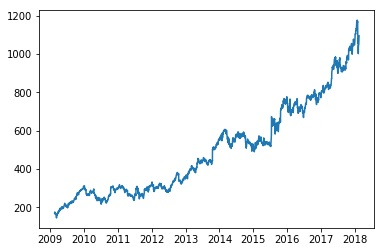
\includegraphics{./figures/1.jpg}
\caption{image alt \textless{}\textgreater{}}
\end{figure}

\begin{itemize}
\tightlist
\item
  Output: Prediction Price at the current day
\item
  Optional output: Suggest Buy/Sell/Hold
\end{itemize}

\section{Solution Statement}\label{solution-statement}

\subsection{Regression Approach}\label{regression-approach}

\begin{itemize}
\tightlist
\item
  Choose Linear Regression for traditional machine learning model
  approach
\item
  For time series Regression, create lagged values as new features
  \[lag(n) = f(t-n) \] \emph{Example}: lagged values with n = 7
\end{itemize}

\begin{longtable}[]{@{}ccccccccc@{}}
\toprule
\textbf{Dates} & \textbf{t} & \textbf{t-1} & \textbf{t-2} & \textbf{t-3}
& \textbf{t-4} & \textbf{t-5} & \textbf{t-6} &
\textbf{t-7}\tabularnewline
\midrule
\endhead
2011-01-08 & 1.020005 & 1.020005 & 1.015140 & 1.007810 & 0.996310 &
1.000000 & 1.00000 & 1.00000\tabularnewline
2011-01-09 & 1.020005 & 1.020005 & 1.020005 & 1.015140 & 1.007810 &
0.996310 & 1.00000 & 1.00000\tabularnewline
2011-01-10 & 1.016315 & 1.020005 & 1.020005 & 1.020005 & 1.015140 &
1.007810 & 0.99631 & 1.00000\tabularnewline
2011-01-11 & 1.019293 & 1.016315 & 1.020005 & 1.020005 & 1.020005 &
1.015140 & 1.00781 & 0.99631\tabularnewline
2011-01-12 & 1.020716 & 1.019293 & 1.016315 & 1.020005 & 1.020005 &
1.020005 & 1.01514 & 1.00781\tabularnewline
\bottomrule
\end{longtable}

\begin{itemize}
\tightlist
\item
  Perform grid search to find the optimal lag order based on Root Mean
  Squared Error(RMSE)
\end{itemize}

\subsection{ARIMA Approach}\label{arima-approach}

\subsubsection{Definition}\label{definition}

\begin{itemize}
\tightlist
\item
  ARIMA stands for Autoregressive Integrated Moving Average (Alternative
  name: Box-Jenkins Model)
\item
  ARIMA is a forecasting technique that projects the future values of a
  series based on its own inertia
\item
  Its main application is short-term forecasting requiring at least 40
  historical data points
\item
  ARIMA works best when data:

  \begin{itemize}
  \tightlist
  \item
    Exhibits a stable or consistent pattern
  \item
    Have a minimum amount of outliers
  \end{itemize}
\end{itemize}

\subsubsection{Models parameter}\label{models-parameter}

\begin{itemize}
\tightlist
\item
  ARIMA attempts to describe the movement in a stationary time series as
  a function of "autoregressive and moving avg"

  \begin{itemize}
  \tightlist
  \item
    AR(autoregressive)
  \item
    MA(moving avg)
  \end{itemize}
\item
  Autoregressive Models:
  \[X(t) = A(1)*X(t-1) + A(2)*X(t-2) +... + A(n)*X(t-n) + E(t)\]

  \begin{itemize}
  \tightlist
  \item
    X(t): the time-series
  \item
    X(t-n): time series lagged n
  \item
    A(n): autoregressive parameters
  \item
    E(t): the error term of the model
  \end{itemize}
\item
  Moving Average Models: \[X(t) = -B(1) * E(t-1) + E(t)\]

  \begin{itemize}
  \tightlist
  \item
    B(1): MA of order 1
  \item
    E(t): current error term
  \item
    E(t-1): error in the previous period
  \end{itemize}
\end{itemize}

\subsubsection{Approach}\label{approach}

\begin{itemize}
\tightlist
\item
  Mixed ARIMA model is built on 3 parameters (p,d,q)

  \begin{itemize}
  \tightlist
  \item
    p: lag order
  \item
    d: degree of differencing
  \item
    q: size of moving average window(order of moving average)
  \end{itemize}
\item
  Perform grid search to find the optimal orders (p,d,q) based on Root
  mean squared error(RMSE)
\end{itemize}

\section{Evaluation Metrics}\label{evaluation-metrics}

\begin{itemize}
\tightlist
\item
  RMSE(Root Mean Squared Error)
  \[RMSE = \sqrt{\frac{\sum_{t \in N}(y_t - \hat{y}_t)^2}{N}}\]
\item
  Reasons to choose RMSE:

  \begin{itemize}
  \tightlist
  \item
    Squaring error to have positive values
  \item
    Putting more weight on large errors
  \end{itemize}
\item
  Cons of choosing RMSE:

  \begin{itemize}
  \tightlist
  \item
    Our data may have many outliers that affect the perfomance
    evaluation
  \end{itemize}
\end{itemize}

\section{Project Design}\label{project-design}

\subsection{Data Exploratory}\label{data-exploratory}

\begin{itemize}
\tightlist
\item
  Perform statical analysis

  \begin{itemize}
  \tightlist
  \item
    Mean
  \item
    Standard Deviation
  \item
    Median
  \item
    Sum
  \end{itemize}
\item
  Visualize time series data

	  \begin{itemize}
	  \item
	    Visualize time-series data \\
	    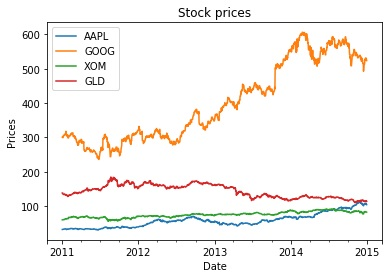
\includegraphics{./figures/2.jpg}
	  \item
	    Bollinger Bands - Rolling stats \\
	    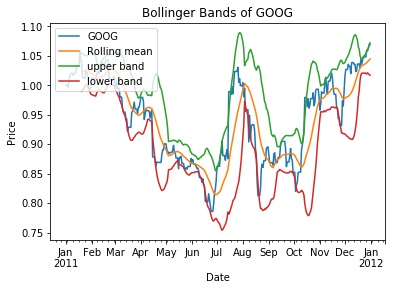
\includegraphics{./figures/3.jpg}
	  \end{itemize}
\end{itemize}

\subsection{Data Preprocessing}\label{data-preprocessing}

\begin{itemize}
\item
  Normalize data \[f(t) = \frac{f(t)}{f(0)}\]
  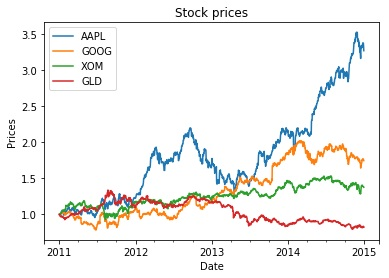
\includegraphics{./figures/4.jpg}
\item
  Remove Trend if nesscessary
\end{itemize}

\subsection{Model Prediction}\label{model-prediction}

\subsubsection{Linear Regression}\label{linear-regression}

\begin{itemize}
\item
  Feature engineering

  \begin{itemize}
  \tightlist
  \item
    Create lagged value
  \item
    Examine correlation between lagged datapoints\\
    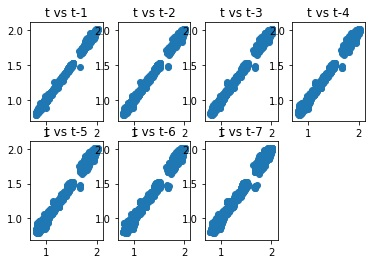
\includegraphics{./figures/5.jpg} 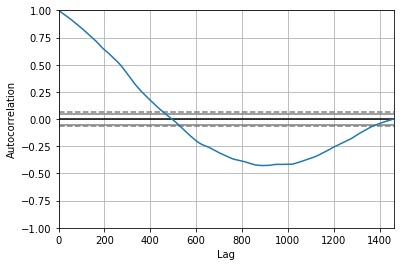
\includegraphics{./figures/6.jpg}
  \end{itemize}
\item
  Split data into trainning/validation/test set\\
  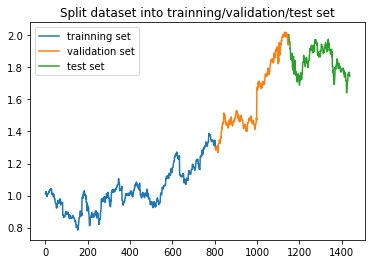
\includegraphics{./figures/7.jpg}
\item
  Perform grid search to find optimal parameters

\begin{Shaded}
\begin{Highlighting}[]
\ControlFlowTok{for}\NormalTok{ lag }\KeywordTok{in}\NormalTok{ lag_values:}
\NormalTok{    model }\OperatorTok{=}\NormalTok{ fit(trainning_set(X, y, lag))}
\NormalTok{    y_hat }\OperatorTok{=}\NormalTok{ model.predict(validation_set(X, lag))}
\NormalTok{    error }\OperatorTok{=}\NormalTok{ RMSE(y }\OperatorTok{-}\NormalTok{ y_hat)}
\NormalTok{    best_params }\OperatorTok{=}\NormalTok{ params }\ControlFlowTok{with}\NormalTok{ minimum error}
\ControlFlowTok{return}\NormalTok{ lag}
\end{Highlighting}
\end{Shaded}
\item
  Evaluate based on RMSE and visualization\\
  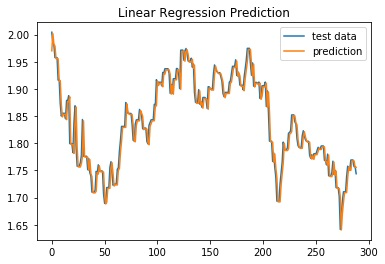
\includegraphics{./figures/8.jpg}
\end{itemize}

\subsubsection{ARIMA}\label{arima}

\begin{itemize}
\item
  Split data into trainning/validation/test set \\
  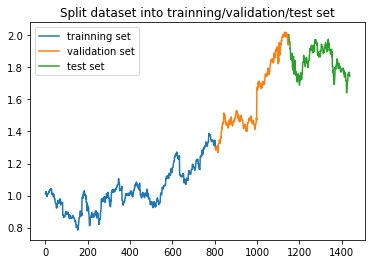
\includegraphics{./figures/7.jpg}
\item
  Perform grid search to find optimal parameters

\begin{Shaded}
\begin{Highlighting}[]
\ControlFlowTok{for}\NormalTok{ each (p,q,d) }\KeywordTok{in}\NormalTok{ order_values:}
\NormalTok{    model }\OperatorTok{=}\NormalTok{ fit(trainning_set(X, y, p, q, d))}
\NormalTok{    y_hat }\OperatorTok{=}\NormalTok{ model.predict(validation_set(X, p, q, d))}
\NormalTok{    error }\OperatorTok{=}\NormalTok{ RMSE(y }\OperatorTok{-}\NormalTok{ y_hat)}
\NormalTok{    best_params }\OperatorTok{=}\NormalTok{ params }\ControlFlowTok{with}\NormalTok{ minimum error}
\ControlFlowTok{return}\NormalTok{ best_params(p,q,d)}
\end{Highlighting}
\end{Shaded}
\item
  Evaluate based on RMSE and visualization
\end{itemize}

\subsection{Model Evaluation}\label{model-evaluation}

\begin{itemize}
\tightlist
\item
  Compare RMSE of 2 different approaches
\item
  Explain the results based on visualizations \\
  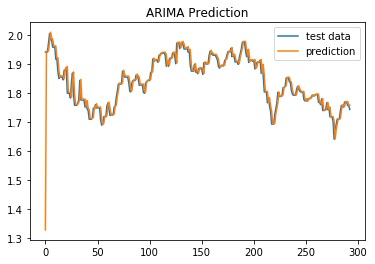
\includegraphics{./figures/9.jpg}
\end{itemize}

\section{Reference}\label{reference}

\url{https://www.quora.com/What-is-ARIMA}


    % Add a bibliography block to the postdoc
    
    
    
    \end{document}
